\documentclass[a4paper,parskip=half]{scrartcl}

\usepackage[T1]{fontenc}
\usepackage[ngerman]{babel}
\usepackage{csquotes}
\usepackage[regular,condensed,sfdefault]{roboto}
\usepackage{graphicx}
\usepackage{chemformula}
\usepackage[backend=biber]{biblatex}
\usepackage[hidelinks,pdfencoding=auto,
  pdfauthor={Thomas Ascher},
  pdfusetitle,
  pdfkeywords={Bier,Kegging,Zapfanlage}]{hyperref}
\usepackage{microtype}

\addto\extrasngerman{
\def\figureautorefname{Abb.}
}

\addto\captionsngerman{
\renewcommand{\figurename}{Abb.}
}

\title{Alkoholmessung mit dem Refraktometer}
\author{Thomas Ascher}

\addbibresource{refraktometer.bib}

\begin{document}
\maketitle

\section*{Einleitung}

\autocite{Terrill2013}
\autocite{Novotny2017}
\autocite{Novotny2017a}
\autocite{Bonham2001}
\autocite{Gossett2012}
\autocite{Gossett2012a}
\autocite{Gossett2012b}
\autocite{Gossett2012c}
\autocite{Troester2012}
\autocite{Terrill2010}
\autocite{Terrill2010a}
\autocite{Terrill2011}
\autocite{Siebel1938}
\autocite{Weiss2016}

%(\autoref{fig:groteblohm}) von 
%Grote \& Bohm \autocite{GroteBlohm2020}.

%\begin{figure}[h]
%\centering
%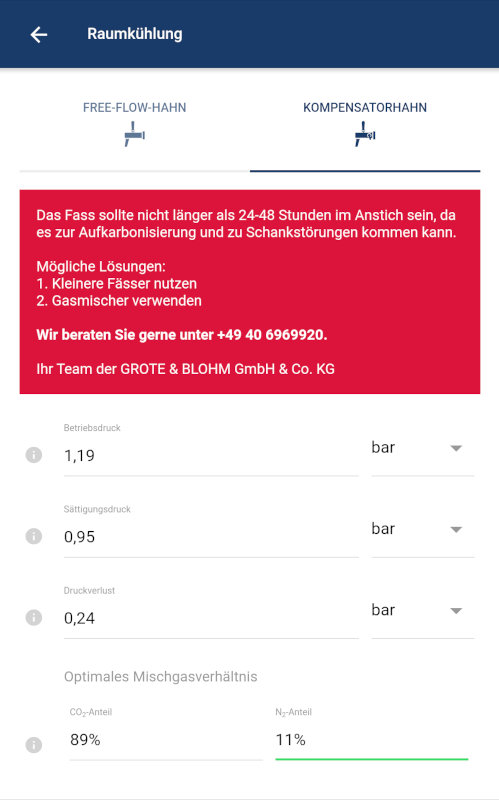
\includegraphics[width=4.8cm]{images/groteblohm.jpg}
%\caption{FOBB-APP}
%\label{fig:groteblohm}
%\end{figure}


\printbibliography[title=Quellen]

\end{document}